\documentclass[tikz,border=8pt]{standalone}
\usepackage{amsmath}
\usetikzlibrary{arrows.meta,positioning,fit}

\begin{document}
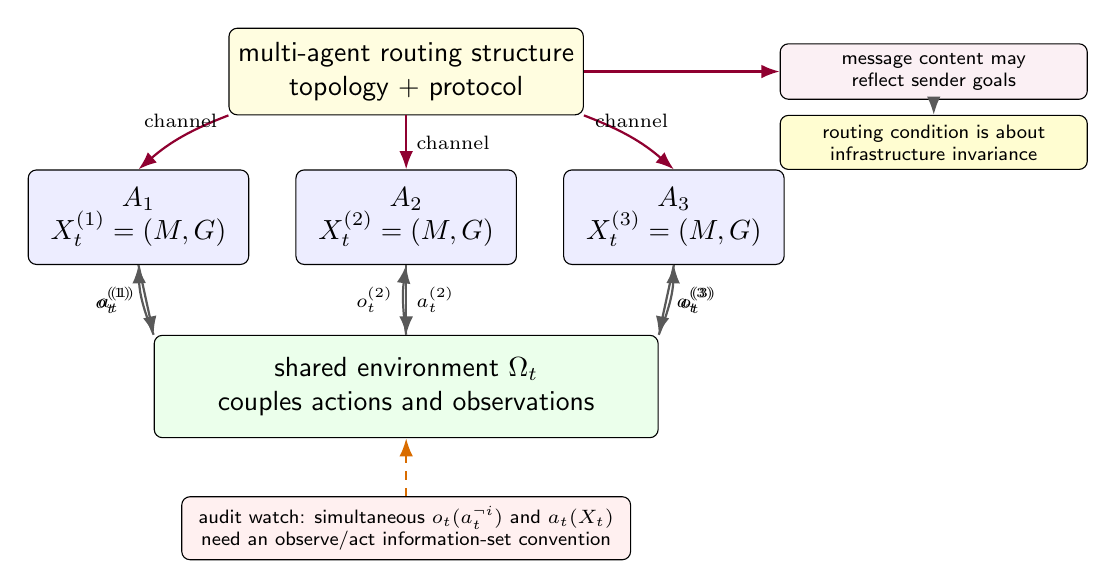
\begin{tikzpicture}[
  font=\sffamily,
  agent/.style={draw, rounded corners=3pt, align=center, minimum width=28mm, minimum height=12mm, fill=blue!7},
  env/.style={draw, rounded corners=3pt, align=center, minimum width=64mm, minimum height=13mm, fill=green!8},
  route/.style={draw, rounded corners=3pt, align=center, minimum width=42mm, minimum height=11mm, fill=yellow!12},
  note/.style={draw, rounded corners=3pt, align=center, font=\sffamily\scriptsize, fill=white},
  arrow/.style={-Latex, thick, draw=black!65},
  msg/.style={-Latex, thick, draw=purple!75!black},
  warn/.style={-Latex, thick, dashed, draw=orange!85!black}
]

\node[agent] (a1) at (-3.4,0.6) {$A_1$\\$X_t^{(1)}=(M,G)$};
\node[agent] (a2) at (0,0.6) {$A_2$\\$X_t^{(2)}=(M,G)$};
\node[agent] (a3) at (3.4,0.6) {$A_3$\\$X_t^{(3)}=(M,G)$};
\node[env] (env) at (0,-1.55) {shared environment $\Omega_t$\\couples actions and observations};

\draw[arrow] (a1.south) -- node[left, font=\scriptsize] {$a_t^{(1)}$} (env.north west);
\draw[arrow] (a2.south) -- node[right, font=\scriptsize] {$a_t^{(2)}$} (env.north);
\draw[arrow] (a3.south) -- node[right, font=\scriptsize] {$a_t^{(3)}$} (env.north east);
\draw[arrow] (env.north west) to[bend left=10] node[left, font=\scriptsize] {$o_t^{(1)}$} (a1.south);
\draw[arrow] (env.north) to[bend left=8] node[left, font=\scriptsize] {$o_t^{(2)}$} (a2.south);
\draw[arrow] (env.north east) to[bend right=10] node[right, font=\scriptsize] {$o_t^{(3)}$} (a3.south);

\node[route] (routing) at (0,2.45) {multi-agent routing structure\\topology + protocol};
\draw[msg] (routing.south west) to[bend right=10] node[above, font=\scriptsize] {channel} (a1.north);
\draw[msg] (routing.south) -- node[right, font=\scriptsize] {channel} (a2.north);
\draw[msg] (routing.south east) to[bend left=10] node[above, font=\scriptsize] {channel} (a3.north);

\node[note, fill=purple!6, minimum width=39mm] (content) at (6.7,2.45)
  {message content may\\reflect sender goals};
\node[note, fill=yellow!18, minimum width=39mm] (infra) at (6.7,1.55)
  {routing condition is about\\infrastructure invariance};
\draw[msg] (routing.east) -- (content.west);
\draw[arrow] (content.south) -- (infra.north);

\node[note, fill=red!6, minimum width=57mm] (timing) at (0,-3.35)
  {audit watch: simultaneous $o_t(a_t^{\neg i})$ and $a_t(X_t)$\\need an observe/act information-set convention};
\draw[warn] (timing.north) -- (env.south);

\end{tikzpicture}
\end{document}
